\chapter{Designed Experimental Protocol to Investigate the Concepts of Variable Recruitment and Co-contraction in Series-viscoelastic Actuators} \label{appendixB}

\section{Aims and Objectives}

\subsection{Aim:}

Characterize the performance of a motor-based tendon driven actuator, intended to assist the knee joint, when series/parallel elasticity is added to it.

\subsection{Objectives:}
\begin{itemize}
    \item Evaluate the performance of the actuator without series/parallel elasticity (rigid) when displacing a hanging load with a sinusoidal trajectory.
    \item Evaluate the performance of the rigid actuator implementing the concept of variable recruitment when displacing a hanging load with a sinusoidal trajectory.
    \item Evaluate the performance of the actuator with series/parallel elasticity (SPEA) when displacing a hanging load with a sinusoidal trajectory.
    \item Evaluate the performance of the SPEA implementing the concept of variable recruitment when displacing a hanging load with a sinusoidal trajectory.
\end{itemize}

\section{Methodology}

An assistive device must provide around 50\% of the peak torque of the assisted joint. The required peak torque and angular speed range for the knee joint during normal walking is 29 Nm and $\pm$50 rpm respectively \cite{dos2014impedance,winter2009biomechanics}. Therefore, the required peak torque to be delivered is 18 Nm. The previous parameters will be used as guidelines when selecting th electric motor/gearbox combination to be used in the experiments.
The experiments to be performed are inspired in the human muscle functionality. In this context, there is a very common configuration based on the human muscles that function in pairs, such as the biceps/triceps pair, also called agnostic/antagonistic configuration. The basic functionality of these muscles is as follows: when the biceps contracts, the triceps relaxes to allow motion in one direction. Similarly, when the triceps contracts, the biceps relax. In real activities, the muscles cooperate with each other to displace a load, this principle is called co-contraction.


\section{Experiment 1}

There are several implementations of the agnostic/antagonistic configuration. In this experimental protocol we are focusing on the simplest one involving co-contraction, i.e. collaboration of the actuators when displacing a load. The first experimental setup (\Cref{fig:setup1}) consists of two actuators (tendon-driven electric motors) controlling a single joint via pulling forces in both directions. This configuration allows the maximum applied torque to be the sum of both motors peak torque. Two main aspects are to be observed in this experiment: 

\begin{itemize}
    \item Synchronous co-contraction via sinusoidal wave input
    \item Stiffness variation via activation of both motors with opposite direction of rotation and different torque amplitudes
\end{itemize}

\begin{figure}[hbt!]
    \centering
    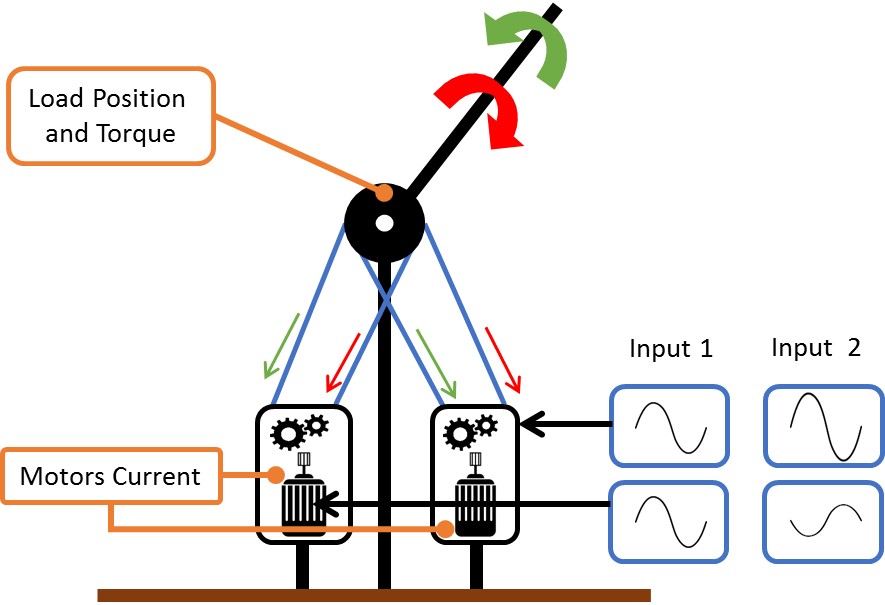
\includegraphics[width=0.8\textwidth]{Setup1.png}
    \caption{Experimental setup 1. Two electric motors work together to create the co-contraction effect in the joint. The required instrumentation is highlighted in yellow. Two different inputs are provided, and the actuator's performance observed.}
    \label{fig:setup1}
\end{figure}

\section{Experiment 2}

The second experiment intended to evaluate the process in which the human muscles recruit several fibres sequentially depending on the desired load. This process is called variable recruitment and has been already implemented in a SPEA with metallic springs as the elastic element \cite{mathijssen2014variable}. In this experiment, the flexion and extension motion of the rigid link is performed by groups of several motors instead of a single one. Therefore, the required peak torque $T_p$  to be delivered is divided among all the participating motors, as described in \Cref{tab:table1}. At the beginning of this section it was mentioned that the total peak torque $T_p$   delivered by the motors must be 50\% of the knee joint peak torque during normal walking, i.e. 18 Nm. The latter means, that for a group composed of two motors, each of them must deliver 50\% of $T_p$. The latter is better described in \Cref{tab:table1}.

\begin{table}[hbt!]
    \centering
    \begin{tabular}{ccc}
    \toprule
    Participating motor & Desired Peak Torque   & Torque per motor\\
    \hline
        2   &  $T_p=$18Nm   & 9 Nm\\
        4   &  $T_p=$18Nm   & 4.5 Nm\\
        6   &  $T_p=$18Nm   & 3 Nm\\
        8   &  $T_p=$18Nm   & 1.5 Nm\\
    \bottomrule
    \end{tabular}
    \caption{Torque requirements for each individual motor in relation to the number of participating motors in the task. The actuator's peak torque $T_p=$18Nm is based on the 50\% of the knee joint peak torque (29 Nm).}
    \label{tab:table1}
\end{table}

For this experiment, it is necessary for the actuators to be back-drivable and to function in their most efficient region (torque-speed). Initially, the first pair of motors in the activation sequence will attempt to displace the load by applying a torque. When the required torque is higher than the maximum allowable torque of the active motor, a second motor in the activation sequence will aid the load displacement. Therefore, the number of active motors in the sequence is entirely dependent on the required torque. The variable recruitment approach allows the motors to operate in a smaller range of speeds, which if carefully selected, ensure the motors to operate in their most efficient region. This is not the case when implementing a single motor which has to comply with a broad range of torques and speed. Therefore, great energy savings potential can be obtained from the variable recruitment approach. The experimental setup is illustrated in \Cref{fig:setup2}. It is important to mention that when a motor is in OFF state it must be back-drivable.

\begin{figure}[hbt!]
    \centering
    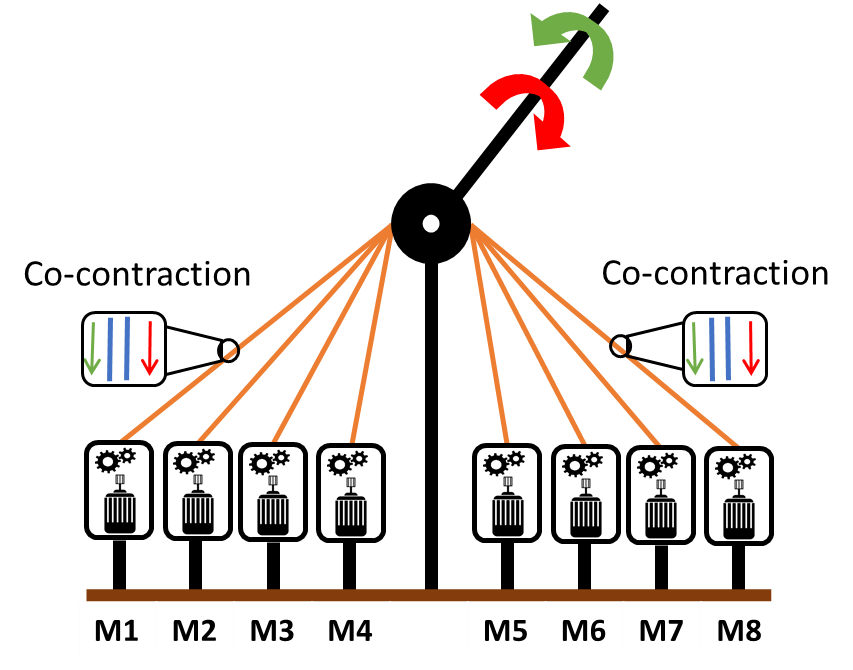
\includegraphics[width=0.8\textwidth]{Setup2.png}
    \caption{Experimental setup 2. Several motors activate in pairs to create co-contraction of the rotating joint. For the sake of clarity in the illustration, the two Bowden cables of each motor are grouped into a single orange cable.}
    \label{fig:setup2}
\end{figure}

\section{Experiment 3}

This experimental setup is the same as in experiment 1 with the only variation of including an elastic element in series with the rotating link (\Cref{fig:setup3}), creating a SPEA. The elastic element is composed of several fibres from the mentioned soft materials. Depending of the stiffness of each soft material, the number of fibres in the elastic element will change taking as reference the recommended optimal stiffness for knee assistance applications. 

\begin{figure}[hbt!]
    \centering
    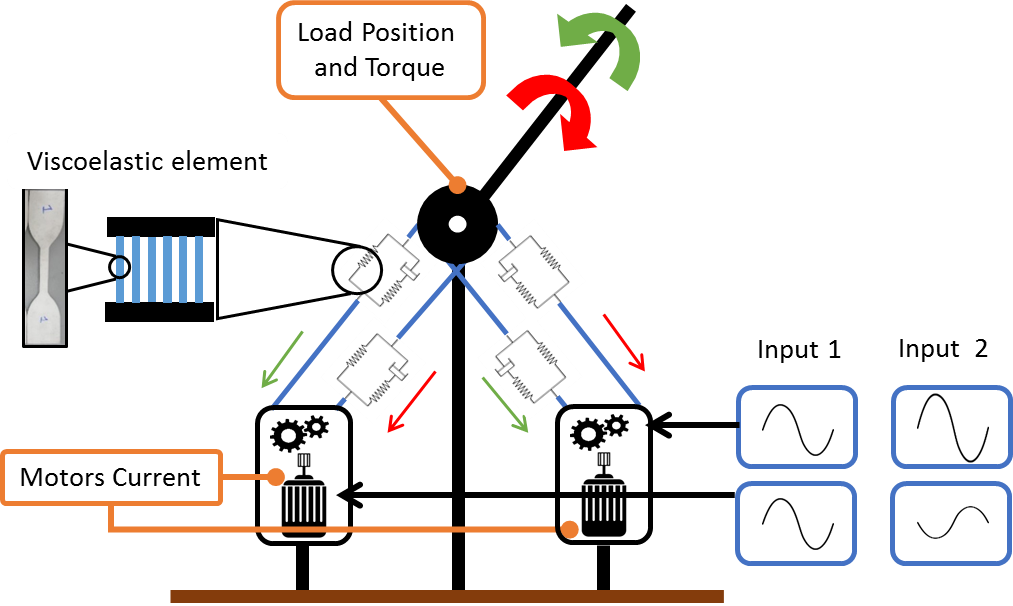
\includegraphics[width=0.8\textwidth]{Setup3.png}
    \caption{Experimental setup 3. Same as in experiment 1 with the only variation of including a viscoelastic element in series with the rotating link.}
    \label{fig:setup3}
\end{figure}

\section{Experiment 4}

Similarly to experiment 2, the variable recruitment approach will be tested using the soft materials. In this case, it is expected a more complex behaviour caused by the deformation of the viscoelastic element and its time dependent properties. The latter will also affect the frequency bandwidth in which the motor is able to transmit the desired torque to the load. The same combinations of motors as in experiment 2 will be used (\Cref{tab:table1}). The experimental setup is illustrated in \Cref{fig:setup4}.

\begin{figure}[hbt!]
    \centering
    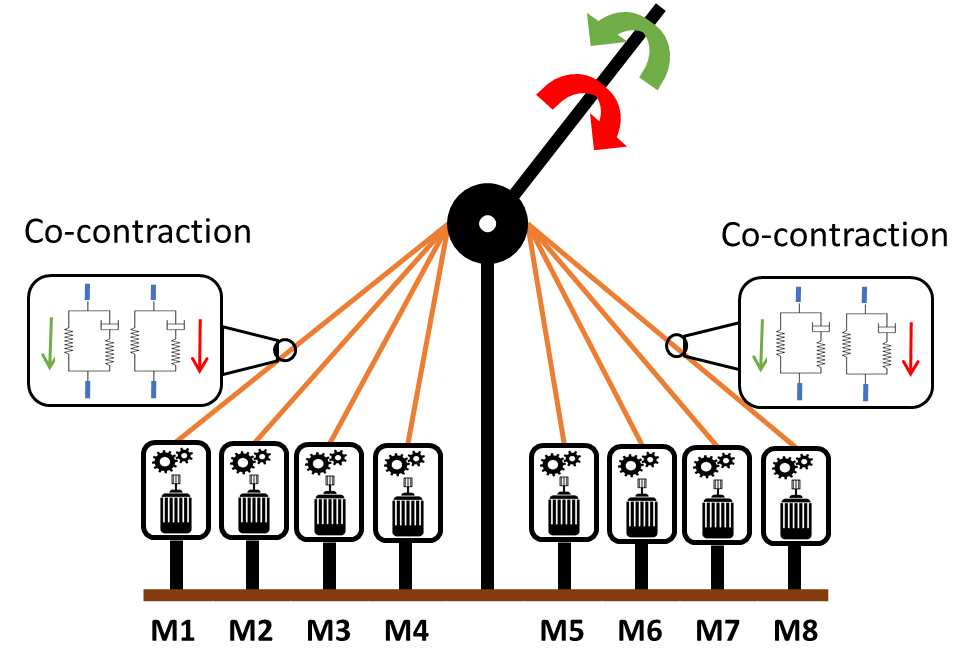
\includegraphics[width=0.8\textwidth]{Setup4.png}
    \caption{Experimental setup 4. Same as in experiment 2 with the only variation of including a viscoelastic element in series with the rotating link.}
    \label{fig:setup4}
\end{figure}
